% %%% fs-state-model - Model

\label {fs-model-section}

In this section, we outline the lightweight deterministic model called {\em drifting state}. While it is described in details in~\cite{we2018adbis}, in this paper we mention properties, which play important roles in consistency enforcement techniques.

We start with basic concepts that allow achieving determinism within a pure streaming engine. Model in terms of the proposed formal framework is described at the end of the section.

Determinism can be achieved in a stream processing system with the following straightforward approach:
\begin{enumerate}
    \item Preserve predefined total order of elements before each non-commutative operation in a data flow
    \item Preserve the same order of output items
    \item Require all operations to be pure
\end{enumerate}

The order on elements can be defined using a natural order of   arrival of input elements. Let us denote it as $t(x)$, $\forall \tau \in \mathbb{N}, a_\tau :  t(a_\tau)=\tau$. The way how $t(x)$ is propagated when an element is transformed into a new one in data flow operations is detailed in section~\ref{ops}.

Drifting state model allows us to efficiently achieve total order enforcement. An underlying idea of the drifting state is a reduced set of available operations which are pure and allow a system to deliver output elements as all computations were in order. On the other hand, these operations are sufficient to implement any stateful streaming computation.

\subsection{Basic operations}
\label{ops}

Any logical graph in the drifting state model is constructed using the following two operations:

{\bf Map} applies a user-defined function to an input item. It returns a sequence of new data items generated from the input. An output sequence can be empty. If $x\in \Gamma$ is an input element of map and $y\subset \Gamma$ is an output one, then $\forall y_i \in y : t(y_i)=t(x)$. The exact ordering between $y_i$ is detailed in~\cite{we2018adbis}.

{\bf Windowed Grouping} stores all input elements sorted by $t(x)$. On each new input element it returns a {\em tuple} that contains sliding window of the last in terms of $t(x)$ elements. The mechanisms that prune groping elements are discussed further. If $(c,d,e)\in \Gamma$ is a tuple element that contains elements $c,d,e \in \Gamma$, then $t((c,d,e))=max(t(c),t(d),t(e))$. 

The following example illustrates the semantics of the operation. The grouping accepts items represented as natural numbers: 1,2,3, etc. If the window is set to 3, the output elements are:

\[(1), (1|2), (1|2|3), (2|3|4), (3|4|5), (4|5|6), (5|6|7), (6|7|8)...\]

\subsubsection{Functional completeness}

Any stateful transformation can be expressed as a composition of a map, a grouping with window size 2, and a cycle. This property is detailed in~\cite{we2018adbis}, and in this paper, we aim to provide an intuitive notion. Let us illustrate it by the example of sum operation. In a typical setting, each element is combined with previous state value and released. Then, the state is updated. In our model, firstly, each element is grouped with previous state element into the pair. After that, map operation delivers a combined result, updates the state, and returns it to the grouping through the cycle. Classical state handling approach is shown in Figure~\ref{classical-drifting}, while drifting state model is demonstrated in Figure~\ref{classical-drifting2}. In drifting state element 4 is grouped with an initial state 0 into the tuple item (0;4). Map operation aggregates tuple element into the new state 4 using sum operation. The state is returned to the grouping through a cycle. After that, input element 3 is grouped with a new obtained state 4. On the next step tuple (4;3) is aggregated into the new state 7 that again is returned to the grouping.   

\begin{figure}[htbp]
  \centering
  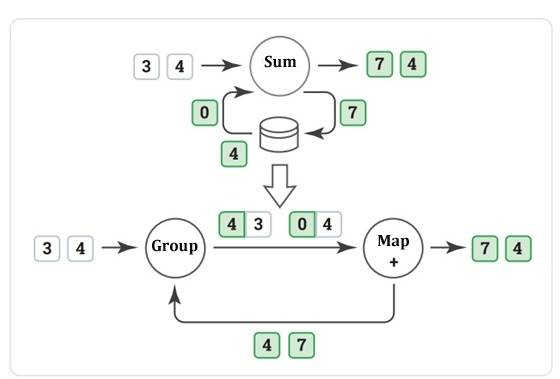
\includegraphics[width=\columnwidth]{pics/classical-drifting}
  \caption{Typical state handling approach}
  \label {classical-drifting}
\end{figure}

\begin{figure}[htbp]
  \centering
  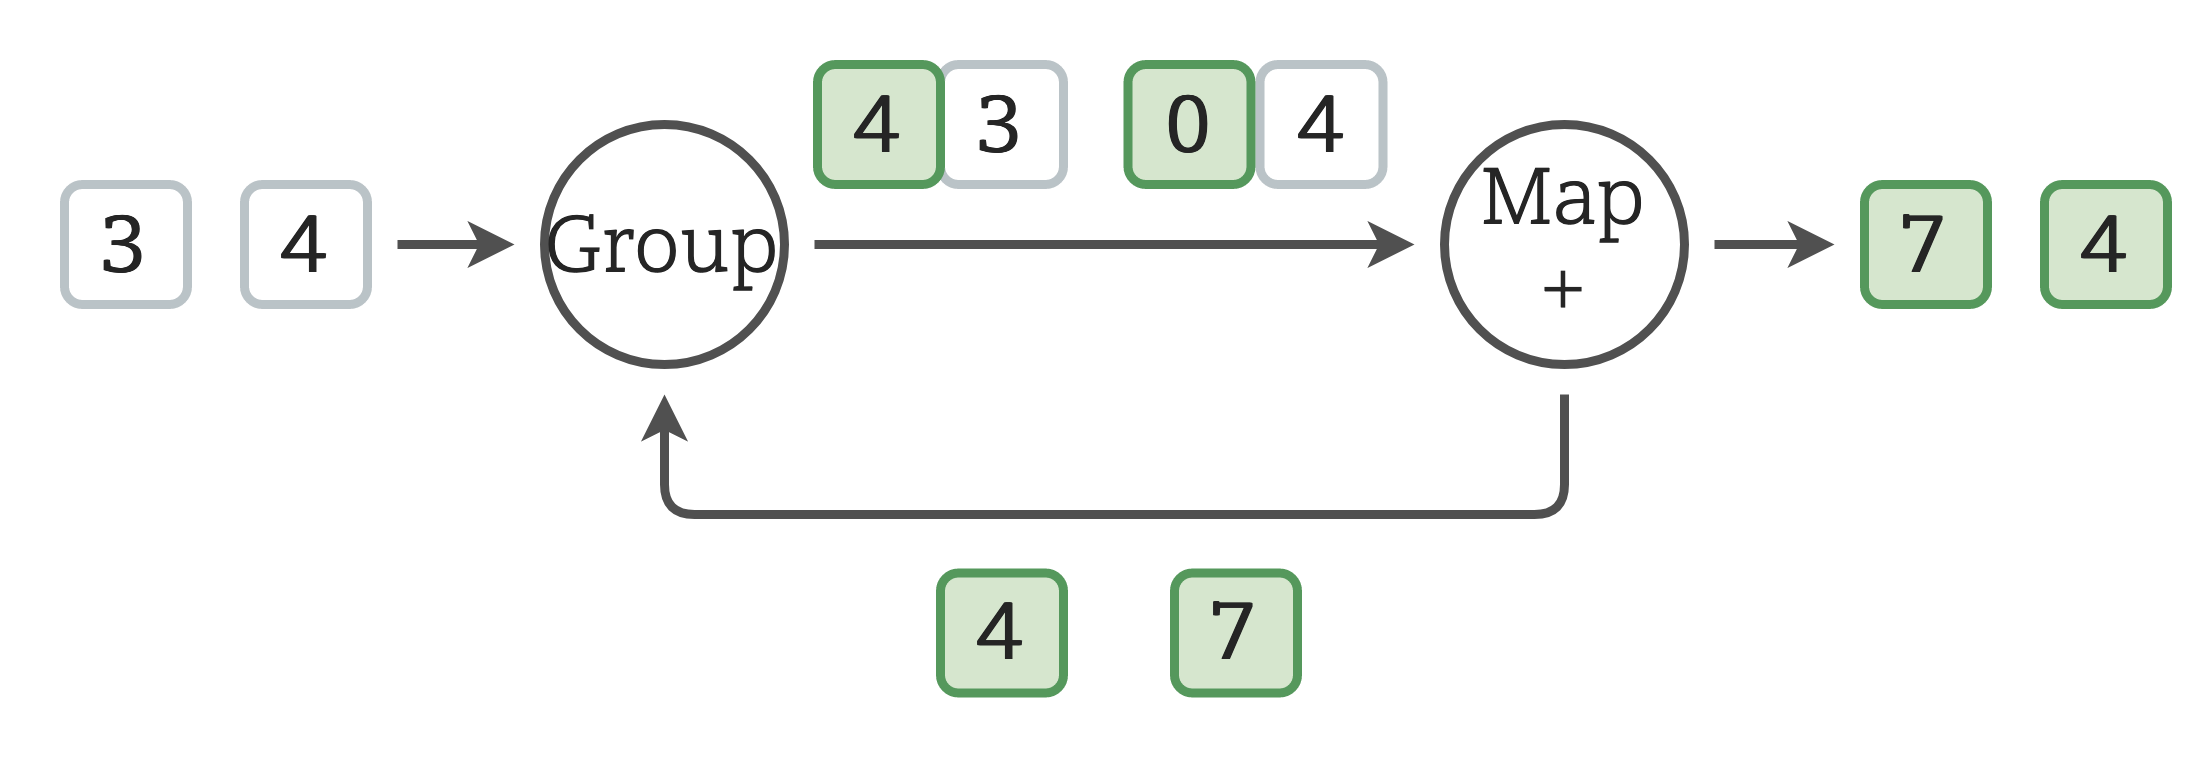
\includegraphics[width=\columnwidth]{pics/classical-drifting2}
  \caption{Drifting state model}
  \label {classical-drifting2}
\end{figure}

\begin{equation}
  \label{flink-contract}
  B(x, h) = y \qquad\Longrightarrow\qquad B(x, s_{\tau}) = (y, s_{\tau+1}) 
\end{equation}

We call this model a drifting state because operation states become ordinary data flow elements. Unlike a common approach, in this model user does not have direct access to state, and state management is done completely on the system side. Let $B$ denote a business logic operation, $x, y$ be input and output items $(x,y)\in D$. Let $h$ be the state handler and $s_\tau$, the state of operation $B$ at time $\tau$. The change in contract is illustrated in (\ref{flink-contract}). In general, such representation of any stateful operation allows us to use {\em binary relations} in the formal framework instead of operations graph.

\subsubsection{Properties}

In this setting, map operation is pure and order insensitive, and grouping operation is pure. Grouping operation is order-sensitive because it should group a new element with the exact previous state. Hence, a straightforward approach to achieve determinism is to enforce order before each grouping in a data flow. Fortunately, grouping can be implemented optimistically, i.e. it can handle out-of-order elements without blocking but possibly generating invalid output. The scheme is shown in Figure~\ref{optimistic-grouping}. The numbers on this figure represent $t(x)$. An arriving element with $t(x)=2$ is out-of-order. We know that invalid pair (1; 3) has been already released. In this case, the system generates valid pairs because the right position of the element 2 is determined. Besides, an invalid pair with a special flag is resent. Let us call such elements {\em sentinels}. Sentinel is colored red in Figure~\ref{optimistic-grouping}. While sentinels mostly behave as ordinary data items, their purpose is to seek and destroy previously released invalid results and their descendants. Map operations handle sentinels as ordinary elements and results inherit sentinel flag. When a sentinel arrives at a grouping, it forces removing a corresponding invalid element from the bucket. Valid pairs and new sentinels are sent further. Map functions are required to be pure in order to ensure that sentinels will go through exactly the same route as original elements. An important property of invalid elements and corresponding sentinels is that they depend on the same input elements. This method is applicable to any number of subsequent groupings and guarantees that all groupings will eventually have such state as if all elements were in-order~\cite{we2018adbis}.
 
\begin{figure}[htbp]
  \centering
  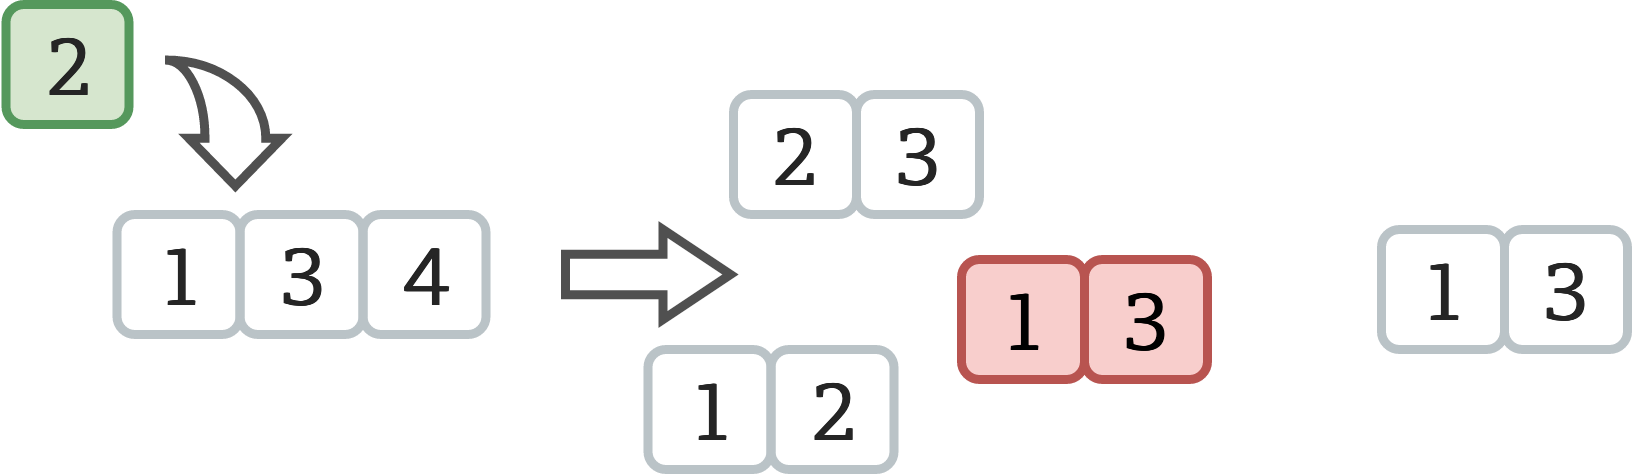
\includegraphics[width=\columnwidth]{pics/grouping-invalidation}
  \caption{An idea of optimistic grouping implementation}
  \label {optimistic-grouping}
\end{figure} 

\subsection{Dependency tracking}

Invalid grouping items must be destroyed by sentinels to prevent inconsistent output. Hence, the system must hold invalid elements before releasing to end-user until all corresponding sentinels arrive. In drifting state model all output items are buffered in the very last node of the logical graph called {\em barrier}. The problem here is to detect that there are no in-flight sentinels for elements in the barrier and they will not be eventually generated. Invalid items and corresponding sentinels always depend on the same input element. Hence, if a system knows that all elements that depend on an input item are in the barrier, these elements can be delivered to end-user. 

Barriers require mechanisms for detecting dependencies between data flow elements. The well-known solution for dependency tracking is to inject special elements in a data flow. These elements go through the same path in a physical graph and "push through" preceding data flow elements. When such element arrives at the barrier, it means that buffered elements do not have in-flight dependencies. Flink checkpointing technique is based on this approach~\cite{Carbone:2017:SMA:3137765.3137777}. While it works well in systems that support only acyclic execution graphs, it is unclear how to handle such "pushing" elements in drifting state cycles. 

To solve this problem, we adopt an idea of {\em Acker} from Apache Storm~\cite{apache:storm}. On each input item, an operation in a physical graph sends to the special agent called~{\em \Acker\ } $t(x)$ together with checksum hashes of the input and output items. \Acker\ XORs all checksums grouped by ranges of $t(x)$ and when the result becomes zero, it means that all items with $t(x)$ in a given interval were processed. In other words, there are no in-flight elements with a given range of $t(x)$, so sentinels with these $t(x)$ will not be generated. When such event occurs, \Acker\ broadcasts a notification that contains the interval of $t(x)$ to the subscribers, e.g. barriers. In this approach, collisions are possible, but they are very unlikely in practice.

Figure~\ref{acker} illustrates~\Acker\ functionality. Different shapes mean different data items. Each operation sends an ack for transformed items before ack for the input one to prevent XORed value become zero until all dependencies are in the barrier. Entries for $t(x) \in [0;5) \cup ... \cup [15;20)$ are zero, so it means that all elements with $t(x)$ in the range $[0;20)$ can be released from the barrier. However, there are still in-flight elements with $t(x) \in [20;25)$, so elements with $t(x) \geq 23$ must not be send out from the barrier.

\begin{figure}[htbp]
  \centering
  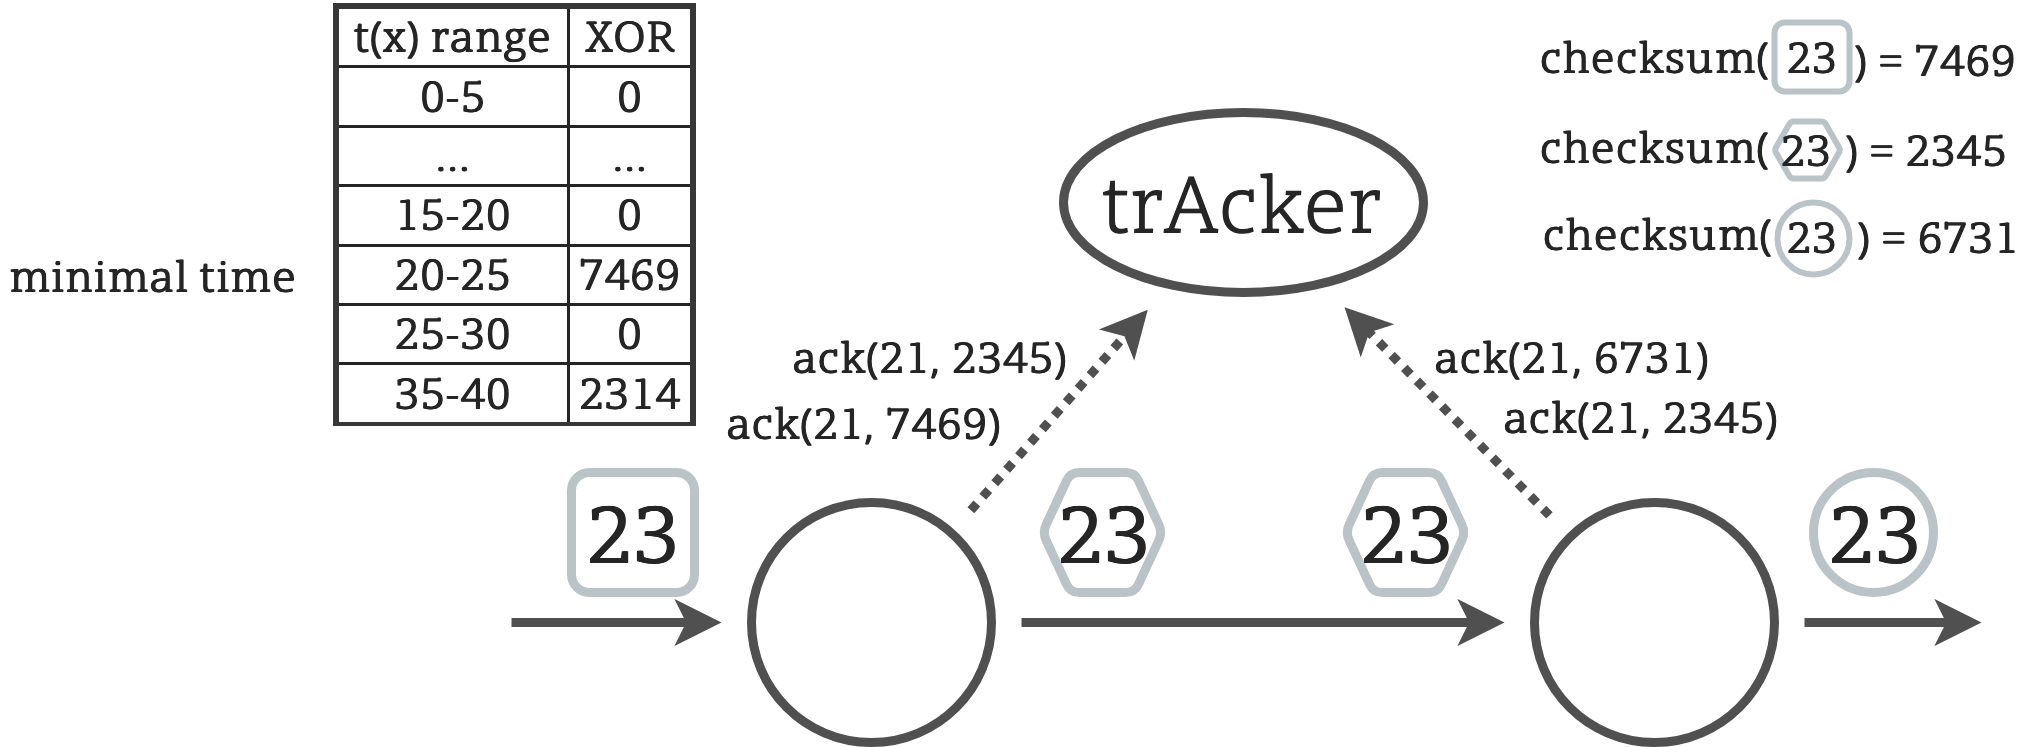
\includegraphics[width=\columnwidth]{pics/acker}
  \caption{The example of tracking dependencies using~\Acker\ }
  \label {acker}
\end{figure}

\subsection{Formal framework model}

According to the formal framework introduced above, the set of data flow elements in drifting state model consists of {\em data items}. Each data item contains user data called {\em payload} and $t(x)$ that defines order.

$$DataItem=(Payload,Meta \ni t(x))$$

Dependency relation $D$ is defined in the form of a possibly cyclic graph containing only map and grouping operations. The drifting state has the following important properties:

\begin{itemize}
    \item Total order enforcement and determinism with only a single buffer at the end of the data flow
    \item States of user operations are ordinary data items
    \item There is only a need to restore grouping buckets to recover processing 
\end{itemize}

Recovery mechanisms for drifting state model are detailed in the next section.